%  section on run scenarios

% CHAPTER ON ILC RUNNING SCENARIOS

One of the key advantages of $e^+e^-$ colliders is the ability to collect individual datasets at specific center-of-mass energies and beam polarisation settings, according to the neeeds of the various physics measurements.
While each measurement has its prefered data-taking mode, the combination with datasets collected at other beam energies and/or beam polarisations provides a unique robustness against systematic uncertainties.

Any physics projection will depend on the exact running scenario, i.e.\ the ensemble of the integrated luminosities collected at the individual center-of-mass energies with the various polarisation settings. The interplay between different datasets has been studied in detail in~\cite{Barklow:2015tja}, with a special focus on the optimisation of the Higgs precision measurements, resulting in a standard running scenario for ILC physics projections. The time evolution of this running scenario has been adapted to the staged construction of the ILC as first presented in~\cite{Fujii:2017vwa}. In this section,
the current understanding of ILC operating scenarios will be summarized based on these references.  


\subsection{Center-of-mass energies and integrated luminosities}
The three center-of-mass energies best motivated by current knowledge have been included in detailed run plans for the ILC spanning about 20 years in real-time:
\begin{itemize}
\item $\sqrt{s}=250$\,GeV for collecting data near the threshold of the Higgsstrahlungs process, 
\item $\sqrt{s}=350$\,GeV for scanning the onset of top-quark pair production, and 
\item $\sqrt{s}=500$\,GeV or somewhat above for studying $t\bar{t}$ production in the continuum and enabling $t\bar{t}H$ and $ZHH$ production. 
\end{itemize}
Table~\ref{tab:lumiabstot} compares the total integrated luminosities foreseen at these energies for three alternative running scenarios to the integrated luminosities assumed in the Snowmass community study. Since 2015, the scenario H-20 is the standard assumption
for ILC physics projections.

\begin{table}[h]
\centering
  \renewcommand{\arraystretch}{1.10}
\begin{tabularx}{\columnwidth}{*{4}{>{\centering\arraybackslash}X} || *{1}{>{\centering\arraybackslash}X}} 
%\begin{tabular*}{\textwidth}{@{\extracolsep{\fill}}c|c c c c c}
%\begin{tabular}{|l||c|c|c|c|c|}
\hline
            &  \multicolumn{4}{c}{$\int{\mathcal{L} dt}$ [fb$^{-1}$]} \\
\hline
$\sqrt{s}$  & G-20      &   H-20   &  I-20   & Snow   \\
\hline
250\,GeV    &  500      &  2000    &   500   & 1150   \\
350\,GeV    &  200      &   200    &  1700   &  200  \\
500\,GeV    & 5000      &  4000    &  4000   & 1600  \\
\hline
%\end{tabular*}
\end{tabularx}
\caption{Proposed total target integrated luminosities for $\sqrt{s}=250$,  $350$, $500$\,GeV based on $20$ ``real-time'' years of ILC operation under scenarios G-20, H-20 and I-20. The total integrated luminosities assumed for Snowmass
are listed for comparison based on 13.7 ``real-time'' years. From~\cite{Barklow:2015tja}}
\label{tab:lumiabstot} 
\end{table}


It must be stressed, however, that flexibility in the running option remains one of the key assets of the ILC, and that it can be adjusted whenever new insights, e.g.\ discoveries at the (HL-)LHC or the ILC itself, require to do so. Thereby, the center-of-mass energy of the ILC can always be lowered from the nominal maximum energy without loss of efficiency and/or luminosity, as long as the electron beam energy remains sufficiently high for positron production. On the contrary, the operation of the SCRF cavities below the maximum gradient
saves significant cryogenic and RF power, which can be invested into higher luminosity!

Future $e^+e^-$ colliders could also provide important physics measurements at other center-of-mass energies. Their priority, however, seems today somewhat lower than for the abovementioned three energies. Therefore they are not explicitely included in the run plan of the ILC or in the current machine design. Nevertheless, Tab.~\ref{tab:lumiabstot1TeV} lists target integrated luminosities recommended for physics studies at these additional energies.

\begin{table}[h]
\centering
  \renewcommand{\arraystretch}{1.10}
\begin{tabularx}{\columnwidth}{l *{4}{>{\centering\arraybackslash}X}} 
%\begin{tabular*}{\textwidth}{@{\extracolsep{\fill}}c|c c c c c}
%\begin{tabular}{|l||c|c|c|c|c|}
\hline
$\sqrt{s}$  &    1\,TeV     &  90\,GeV & 160\,GeV  \\
\hline
 $\int{\mathcal{L} dt}$ [fb$^{-1}$]           & 8000 	   &  100       &  500  \\
\hline
%\end{tabular*}
\end{tabularx}
\caption{Proposed total target integrated luminosities for other $\sqrt{s}$.  From~\cite{Barklow:2015tja}.}
\label{tab:lumiabstot1TeV} 
\end{table}


\subsection{Beam polarisation}

At center-of-mass energies of up to 500\,GeV, the ILC beams are foreseen to be polarised  with absolute values of at least 80\% for the electrons and at least 30\% for the positrons. At 1\,TeV, the positron polarisation will at least reach 20\%. As an upgrade option, the positron polarisation can be increased to 60\%. The accelerator design comprises sets of spin rotators which in principle allow to prepare any desired direction of the polarisation vectors at the IP. However in the detailed running scenarios, only longitudinal polarisation is considered. The sign of the beam polarisations can be flipped 
on a train-by-train basis. This allows to collect data sets with different helicity configurations quasi-concurrently w.r.t.\ changes in the accelerator or detector configuration, calibration and alignment. This allows to construct observables in which
large parts of the experimental systematic uncertainties cancel. A famous example is the traditional left-right asymmetry --- more generally the joint interpretation of the different data sets allows to treat many systematic effects as nuissance parameters in global fits. 


\begin{table}[h]
\centering
  \renewcommand{\arraystretch}{1.10}
\begin{tabularx}{\columnwidth}{l *{4}{>{\centering\arraybackslash}X}} 
%\begin{tabular*}{\textwidth}{@{\extracolsep{\fill}}|c|c|c|c|c|c|}
%\begin{tabular}{|l||c|c|c|c|c|}
\hline
        & \multicolumn{4}{c}{fraction with $\operatorname{sgn}(P(e^-),P(e^+))= $ } \\
           & (-,+) & (+,-) & (-,-) & (+,+) \\
\hline
$\sqrt{s}$ & [\%]  &  [\%] & [\%]  & [\%]  \\ 
\hline
250\,GeV (2015)   & 67.5 &  22.5 &  5    &   5   \\
250\,GeV (update) & \bf{45} &  \bf{45} &  5    &   5   \\
350\,GeV   & 67.5 &  22.5 &  5    &   5   \\
500\,GeV   &  40  &  40   &  10   &  10   \\
\hline
%\end{tabular*}
\end{tabularx}
\caption{Relative sharing between beam helicity configurations proposed for the various center-of-mass energies. The update of the luminosity
sharing fro 250\,GeV originates from the importance of the left-right asymmetry of the Higgsstrahlung cross section in the EFT-based Higgs coupling fit.}
\label{tab:pollumirel} 
\end{table}

\begin{table}[h]
\centering
  \renewcommand{\arraystretch}{1.10}
\begin{tabularx}{\columnwidth}{l *{4}{>{\centering\arraybackslash}X}}    %\begin{tabular*}{\textwidth}{@{\extracolsep{\fill}}|c|c|c|c|c|}
%\begin{tabular}{|l|c|c|c|c|}
\hline
        &  \multicolumn{4}{c}{int. luminosity with $\operatorname{sgn}(P(e^-),P(e^+))= $ } \\
           & (-,+)       & (+,-)       & (-,-)       &  (+,+)     \\
\hline
$\sqrt{s}$ & [fb$^{-1}$] & [fb$^{-1}$] &  [fb$^{-1}$] & [fb$^{-1}$] \\ 
\hline
250\,GeV (2015)   &  1350      &  450        &  100	      &   100  \\
250\,GeV (update) &  \bf{900}  &  \bf{900}   &  100	      &   100  \\
350\,GeV          &   135      &   45	     &   10	      &    10  \\
500\,GeV          &  1600      & 1600        &  400	      &   400  \\
\hline
\end{tabularx}
\caption{Integrated luminosities per beam helicity configuration resulting from the fractions in table~\ref{tab:pollumirel} in scenario H-20. The update of the luminosity
sharing fro 250\,GeV originates from the importance of the left-right asymmetry of the Higgsstrahlung cross section in the EFT-based Higgs coupling fit. 
}
\label{tab:pollumiabs} 
\end{table}

\begin{table}[h]
\centering
  \renewcommand{\arraystretch}{1.10}
\begin{tabularx}{\columnwidth}{l *{4}{>{\centering\arraybackslash}X}} 
%\begin{tabular*}{\textwidth}{@{\extracolsep{\fill}}|c|c|c|c|c|c|}
%\begin{tabular}{|l||c|c|c|c|c|}
\hline
        & \multicolumn{4}{c}{fraction with $\operatorname{sgn}(P(e^-),P(e^+))= $ } \\
           & (-,+) & (+,-) & (-,-) & (+,+) \\
\hline
$\sqrt{s}$ & [\%]  &  [\%] & [\%]  & [\%]  \\ 
\hline
1\,TeV     &  40  &  40   &  10   &  10   \\
90\,GeV    &  40  &  40   &  10   &  10   \\
160\,GeV   & 67.5 &  22.5 &  5    &   5   \\
\hline
%\end{tabular*}
\end{tabularx}
\caption{Relative sharing between beam helicity configurations proposed for low energy and $1$\,TeV running. From~\cite{Barklow:2015tja}.}
\label{tab:pollumirel1TeV} 
\end{table}

\begin{table}[h]
\centering
  \renewcommand{\arraystretch}{1.10}
\begin{tabularx}{\columnwidth}{l *{4}{>{\centering\arraybackslash}X}}    %\begin{tabular*}{\textwidth}{@{\extracolsep{\fill}}|c|c|c|c|c|}
%\begin{tabular}{|l|c|c|c|c|}
\hline
        &  \multicolumn{4}{c}{integrated luminosity with $\operatorname{sgn}(P(e^-),P(e^+))= $ } \\
           & (-,+)       & (+,-)       & (-,-)       &  (+,+)     \\
\hline
$\sqrt{s}$ & [fb$^{-1}$] & [fb$^{-1}$] &  [fb$^{-1}$] & [fb$^{-1}$] \\ 
\hline
1\,TeV      &  3200   	 & 3200        &  800	      &   800  \\
90\,GeV     &    40   	 &   40        &   10	      &    10  \\
160\,GeV    &   340   	 &  110        &   25	      &    25  \\
\hline
\end{tabularx}
\caption{Integrated luminosities per beam helicity configuration resulting from the fractions in table~\ref{tab:pollumirel1TeV}. From~\cite{Barklow:2015tja}.}
\label{tab:pollumiabs1TeV} 
\end{table}


\subsection{Time Evolution and Upgrade Options}
{\color{red} Time dependence: explain why need longer when starting at 250\,\GeV}

{\color{red} explain new beam parameters, cite machine staging report}


%%%%%%%%%%%%%%%%%%%%%%%%%%%%%%%%%%%%%%%%%%%%%%%%%%%%%%%%%%%%%%%%%%%%%%%%%
\begin{figure}
\begin{center}
\includegraphics[width=0.75\hsize]{chapters/figures/lumi_H-20.pdf}
\end{center}
\caption{The nominal 20-year running program for the 500-GeV-ILC~\cite{Barklow:2015tja}.}
\label{fig:H20}
\end{figure}
%%%%%%%%%%%%%%%%%%%%%%%%%%%%%%%%%%%%%%%%%%%%%%%%%%%%%%%%%%%%%%%%%%%%%%%%%%%

%%%%%%%%%%%%%%%%%%%%%%%%%%%%%%%%%%%%%%%%%%%%%%%%%%%%%%%%%%%%%%%%%%%%%%%%%
\begin{figure}
\begin{center}
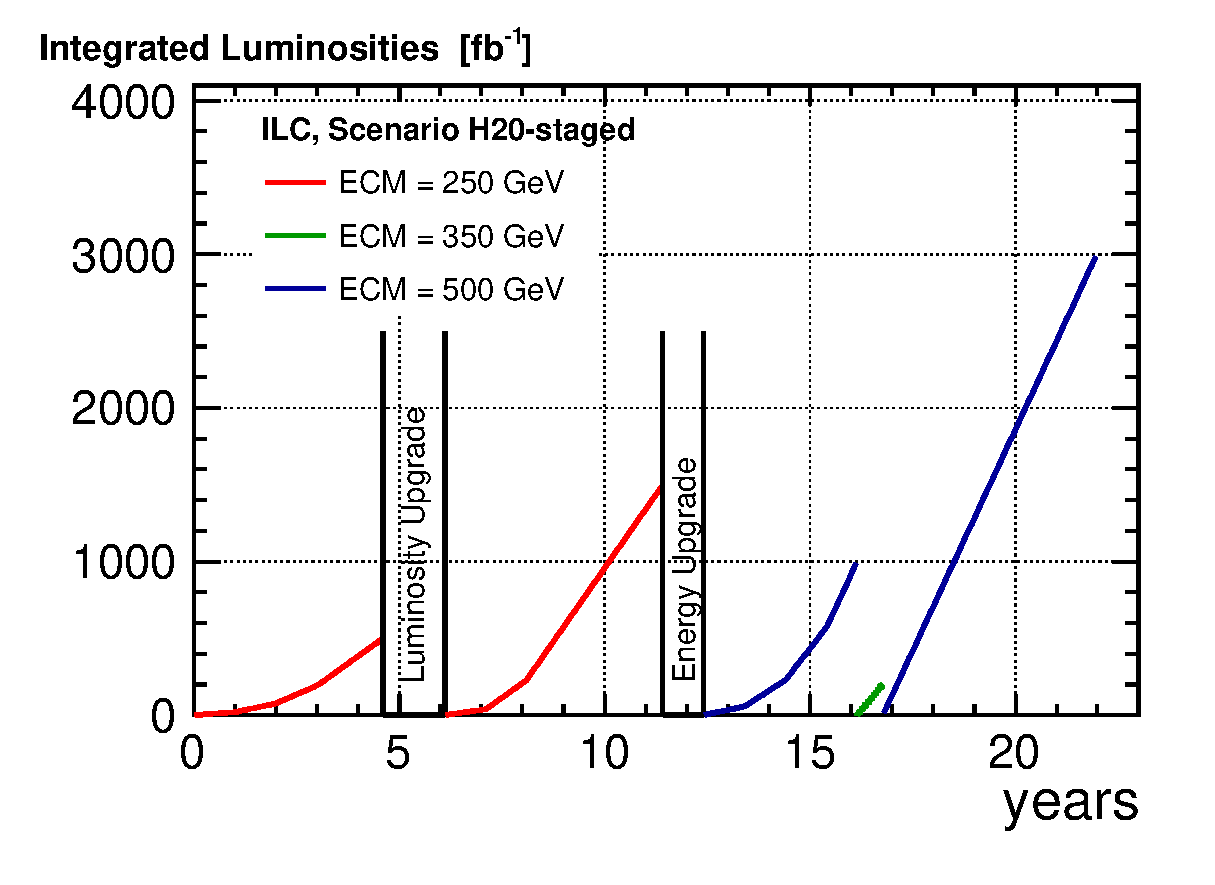
\includegraphics[width=0.75\hsize]{chapters/figures/lumi_H20-staged}
\end{center}
\caption{The nominal 22-year running program for the staged ILC, starting operation at 250\,\GeV ~\cite{Fujii:2017vwa}. The integrated luminosities are the same of for the original H20 scenario.}
\label{fig:H20staged}
\end{figure}
%%%%%%%%%%%%%%%%%%%%%%%%%%%%%%%%%%%%%%%%%%%%%%%%%%%%%%%%%%%%%%%%%%%%%%%%%%%


